\documentclass{IEEEtran}
\usepackage{lettrine}
\usepackage{tabu}
\usepackage{longtable}
\usepackage{tabularx}
\usepackage{amsmath}
\usepackage{graphicx}

\begin{document}
	
\title{Survey of RDBMS vs. Graph Database Performance Using Time Series Data Manipulation}
\author{Paul Marquardt and Kristen Rollins 
\thanks{This paper was submitted for a grade on April 23, 2019. The project was completed under the supervision of Dr. Daniel Engels at Southern Methodist University.} 
\thanks{The authors can be contacted by email: Paul Marquardt at pmarquardt@smu.edu and Kristen Rollins at kmrollins@smu.edu.}}

\maketitle

\begin{abstract}
In this paper, we present a performance evaluation of relational databases and graph databases in the application of calculating a Volatility Index Rating (VIR) using historical stock market data. VIR allows option traders to find the best time to purchase options while volatility is low but stock prices are rising.  VIR is calculated using the formula: VIR = (Highest Close – Current Close) / (Highest High) * 100 over the last twenty-two days of trading.  This requires a calculation of the highest closing price and highest stock bid price for twenty-two days for each stock symbol. Results were varied among both database management system types. 

\end{abstract}

\begin{IEEEkeywords}
	databases, relational databases, MySQL, graph databases, Neo4j
\end{IEEEkeywords}


\section{Introduction}

\lettrine{I}{n} today’s world, there are nearly countless database systems that have been developed and are available to use for a given application. While there may be many accessible programs, we know that different types of database systems are more appropriate to use in some situations than others. One such application that we investigated was the storage and manipulation of time series data, or stock exchange data in particular. In this domain we evaluated multiple database management systems on both suitability and performance. 

To determine the most appropriate DBMS for our domain, we used both MySQL and Neo4j to store stock data, and then use those software systems to manipulate the data and calculate Volatility Index Ratings for many stock symbols. We then compared performance metrics for each respective database system, including DBMS internal metrics as well as OS level metrics such as CPU, RAM, and disk performance statistics. Because of the interrelated nature of time series data, we suspected that a graph database system would provide an efficient and suitable representation for such data. Conversely, we hypothesized that a relational database system would be an inefficient and inappropriate choice for storing and querying time series data. 

Contrary to our hypothesis, we found that Neo4j was not an effective representation of the stock exchange data, and its performance was not better than MySQL for this application. Only one out of three Volatility calculations were completed, while the other two were allowed to run for multiple days but never completed. For this single calculation that was able to finish, MySQL performed slightly better than Neo4j. Our primary conclusion was that both database management systems are inappropriate choices for making the intensive calculations, but between the two, MySQL marginally beats out Neo4j.  

\section{Stock Exchange Data}

In our research, we utilized data from three American stock exchanges. Those were the Amex, Nasdaq, and NYSE exchanges, which are the three largest financial securities markets in the United States. Each company belonging to these markets is identified by a stock symbol, also known as a ticker symbol. This symbol is an abbreviation consisting of letters, numbers, or a combination of the two, and is used to uniquely identify those company shares. Every day, the stock price for every company fluctuates constantly, based on supply and demand for its shares on the market. Stock price data can be collected at any granularity, but only daily stock data is of interest for our purposes. 

For all of these stock symbols, on each trading day the attributes of High, Low, Open, Close, and Volume are recorded. Trading days are typically every Monday through Friday, excluding major holidays. The High value recorded is the maximum price of a company’s stock over the course of a trading day. Similarly, the Low is the minimum value that the stock reached during that day. The stock’s Opening price is the price at which securities are traded when an exchange is opened on a trading day; for example, Amex, the New York Stock Exchange, and the Nasdaq exchange all open at exactly 9:30 a.m. Eastern time. Conversely, the Closing price of a stock is the stock’s value when the exchange is closed for the day, which for Amex, NYSE, and Nasdaq is 4:00 p.m. Eastern Standard Time. The Volume attribute recorded for each symbol is the number of shares that changed hands during that trading day. Using this data, we are able to compute a calculation of interest known as a Volatility Index Rating. 

\subsection{Volatility Index Rating}

The Volatility Index Rating, or VIR, calculation can be made for each symbol for each day. This value is a relative measure of how volatile a company’s stocks are estimated to be on a given day, based on recent trading behavior. This gauge of volatility, when observed closely, can lead to useful insights and profitable trading strategies. Such profits are expected to occur when a company's stock value is observed to be increasing, while the symbol’s VIR is low or decreasing. As indicated in Fig. \ref{fig:vir_example}, in this situation it would be profitable for a trader to purchase stock in that company, as the value is expected to continue increasing in a non-volatile manner. 

\begin{figure}
	\centering
	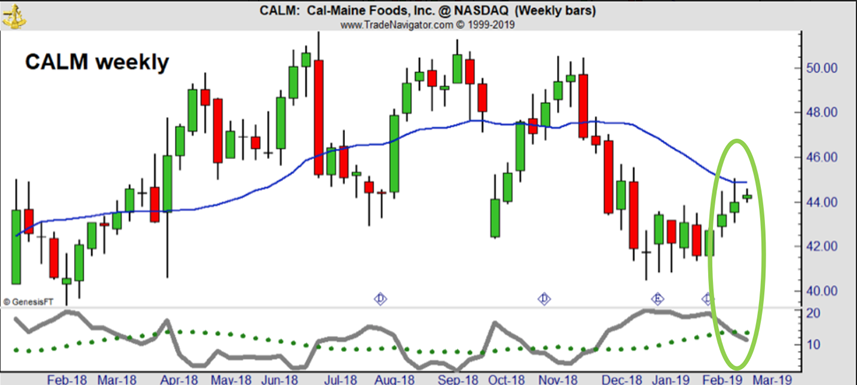
\includegraphics[width=3.5in]{Images/vir_example.png}
	\caption{VIR is shown by the grey line under the stock value fluctuation. The green oval indicates a profitable moment to purchase stock, as the stock value is increasing while the VIR is decreasing.}
	\label{fig:vir_example}
\end{figure}

The formula for VIR on a given day is computed using the symbol's data from the previous 22 days. The calculation is given in Equation \ref{eq:vir}. The resulting value is a percentage, as indicated by the factor of 100 in the equation. 

\begin{equation}
\text{VIR} = \frac{(\text{Highest Close} - \text{Current Close})}{\text{(Highest High)}} \cdot 100 \label{eq:vir}
\end{equation}

In order to store and manipulate stock exchange data and perform this calculation, we must understand and utilize database management systems. Such systems work to let users create and maintain databases, while securely allowing appropriate access to users. Two opposing types of DBMSs are relational and graph databases. We chose these two families of database systems because of their stark differences yet wide-spread use. With these two systems we could store our stock data with differing schemas and strategies, in order to determine which is more appropriate for our application. 

\section{Relational DBMS}

Relational database management systems serve many purposes for applications today. RDBMSs store data in a very structured, pre-defined tabular format. Tables consist of rows or records as well as columns or attributes. Primary keys are used to uniquely identify records, and foreign keys enable relationships between tables. Variations of the programming language SQL, which stands for Structured Query Language, are used to create, retrieve, and manipulate data within the RDBMS. SQL was first developed by IBM in the 1970s, and the relational data model was adopted as the standard method for storing data, and it reigned for a long time. It was not until NoSQL databases were developed that alternatives were available. Because the relational model was the primary database type for several decades, it is used in countless applications today. It is an ideal model for highly structured data, but it often falls short when dealing with highly variable or very large sets of data. The specific relational DBMS we chose to perform our research with was MySQL. This RDBMS is open source and widely used for the needs of many applications.   

\section{Graph DBMS}

Graph database systems take a very different approach than do RDBMSs. These databases are based on graph theory, which is an area of mathematics that studies graphs. In this context, graphs are structures consisting of objects, commonly known as nodes or vertices, which can be connected by edges. These edges can be directed or undirected, and they convey pairwise relationships between objects. Graphs in graph databases are based on these structures, and have corresponding properties. Graph databases are a type of NoSQL database (often interpreted as ‘Not Only SQL’), which were created as a shift away from the inflexible nature of SQL databases and attempt to repair the shortcomings of SQL. NoSQL databases grew to popularity in the late 2000s and have continued to gain traction since. 

We chose Neo4j as our graph DBMS because it is open-source and the most popular graph database system, and thus has a large online community to provide support and resources. Neo4j was first released in 2007, parallel to the rise of NoSQL ideology, and it is currently in its third major release. Corresponding to graphs in graph theory, Neo4j stores its data in nodes. These nodes are simply objects having any number of properties, or key-value pairs. Nodes may also have any number of labels associated with them, which can serve to categorize the data. Neo4j graphs also consist of named relationships, which can connect nodes in a certain direction. While all relationships are directed in Neo4j, multiple relationships can be made between two nodes to convey bi-directionality, and queries can be made to ignore direction. In addition, properties can describe relationships as well as nodes. A simple example of a graph structure that could be stored in Neo4j is found in Fig. \ref{fig:graphdb_ex}. This representation of data can be very powerful and is able to serve the needs of a different class of applications.    

\begin{figure}
	\centering
	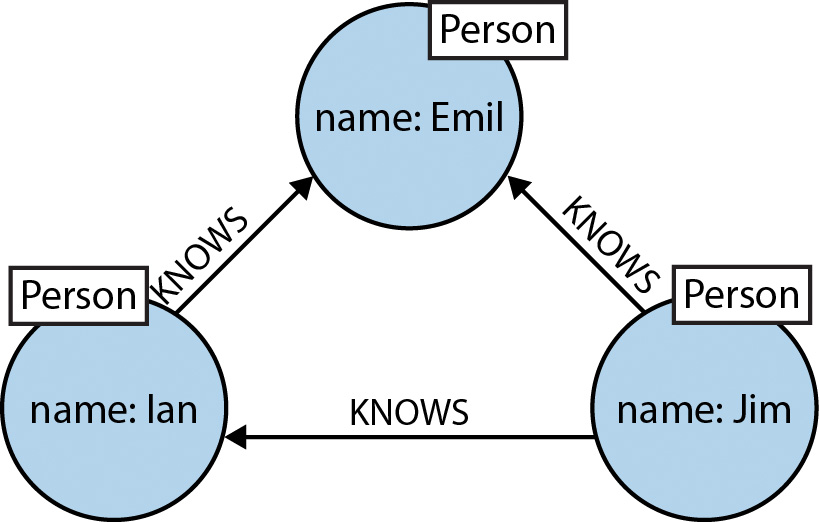
\includegraphics[width=3in]{Images/graphdb_simple_example.jpg}
	\caption{In this simple graph example, the blue circles represent nodes, each having the ``Person" label. All of the nodes have a ``name" property, seen inside each node. The lines between nodes indicate the ``knows" relationship, with the arrow denoting the direction; e.g. Jim knows Ian, and Jim and Ian both know Emil.}
	\label{fig:graphdb_ex}
\end{figure}  

\section{Solution Methodology}

Our overall research approach was to collect sufficient stock data, create data models for both MySQL and Neo4j, calculate the VIR for all stock symbols, and finally run tests to collect and compare various performance metrics. 

\subsection{Data Collection}

To collect adequate stock data for our research, we initially downloaded all of the symbol information for each of the stock exchanges of interest (Amex, Nasdaq, and NYSE) from www.nasdaq.com. We then cleaned up this information and created files consisting of only the ticker symbols for each exchange. 

After procuring these stock symbols, we proceeded to write Python scripts to download daily stock data from Yahoo. These Python scripts utilized the pandas-datareader library, and specified our desired start and end dates. For each day and symbol, the attributes of High, Low, Open, Close, and Volume were recorded. Fig. \ref{fig:raw_data} shows a few lines of raw data that were obtained in this way. In addition, we added an Exchange column to the raw data, indicating which stock exchange each company belongs to.  

\begin{figure}
	\centering
	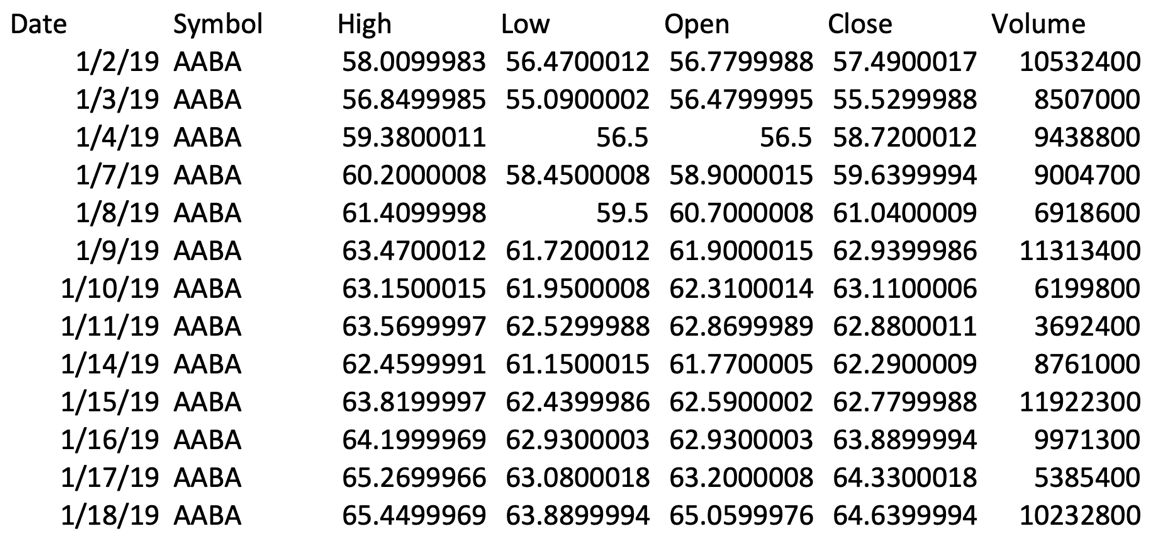
\includegraphics[width=3.5in]{Images/raw_stock_data.png}
	\caption{Slice of raw data obtained from Yahoo daily stock data via Python script.}
	\label{fig:raw_data}
\end{figure}

\subsection{Data Models}

Additionally, we created the data models for both relational and graph database systems. These models served to organize the structure of our data for each DBMS, which was necessary before inserting any data into the databases. 

\subsubsection{MySQL} 

The first data model we created was an Entity-Relational diagram as depicted in Fig. \ref{fig:mysql_model}, in order to format our data for a MySQL database. Tables were created for the daily input of data collected for each exchange, Amex, Nasdaq, and NYSE. Separate tables were created for calculations, AmxReqs, NyReqs, NdqReqs. Indexes are highlighted in yellow.

\begin{figure}
	\centering
	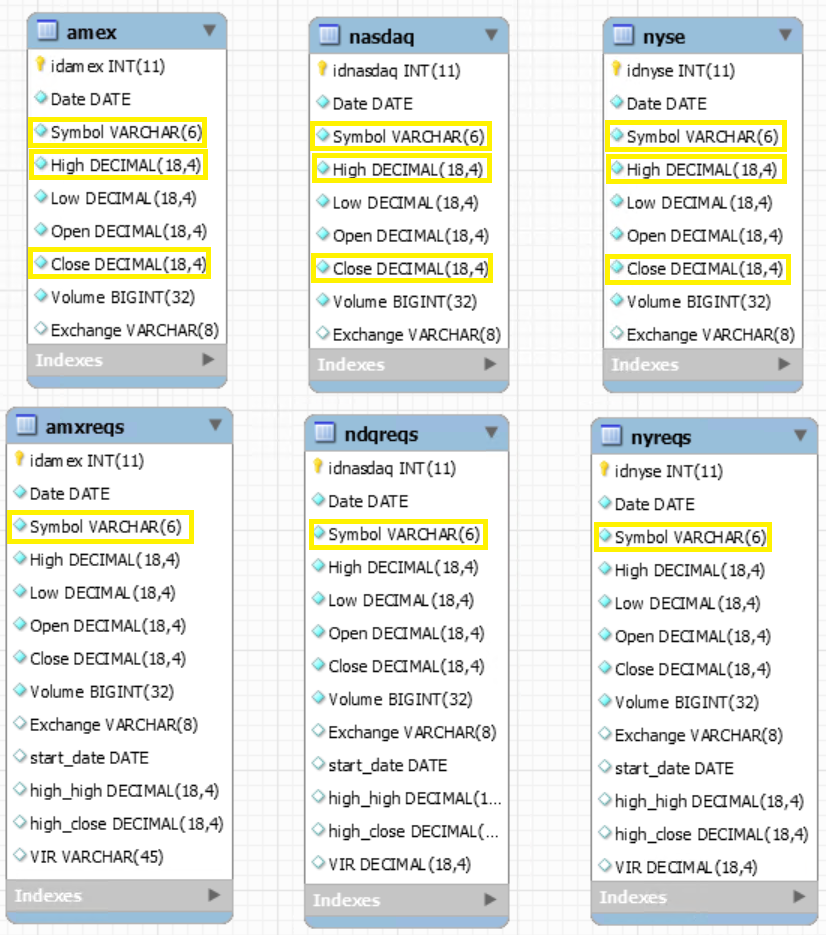
\includegraphics[width=3.5in]{Images/mysql_data_model.png}
	\caption{Data model for MySQL, created in MySQL Workbench. Attributes with indexes are highlighted in yellow.}
	\label{fig:mysql_model}
\end{figure}

Tables were created with the properties shown in Fig. \ref{fig:mysql_model}. Ticker symbols are limited to a six-character maximum to alleviate any unused space. Price data for High, Low, Open, and Close are all decimal values with eighteen digits and four decimal places. This allows for maximization of space and allocates enough decimal space to keep track of minute changes in lower valued securities which trade in one thousandth of a penny.  

Exchange is comprised of a \texttt{varchar} with six characters since our largest exchange value is Nasdaq which is made up of six characters. The ID and primary key for the tables is an integer with eleven characters. This maximizes the scalability of the relational database model by streamlining the amount of data which has to be collected and then processed. Indexes were added to the following columns: Symbol, High, and Close to allow for greater performance during the data calculation queries. 

None of the tables have relationships between them. These tables are used to house the bulk of daily data, then the data is transferred to the requirements tables for calculation: AmxReqs, NdqReqs, NyReqs. The Daily data tables are used for posterity of data collection and are not used for any calculation purposes other than the start\_date of the VIR calculation. 

The second set of tables house the daily information for each of the symbols accompanied by the requirements for calculation of the VIR. The tables are replicated from the corresponding daily tables with added columns for start\_date, high\_high, high\_close, and VIR. Start\_date holds the start date of the twenty second day before the current date to begin the VIR calculation. High\_High houses the highest high value for the previous twenty-two days, and High\_Close houses the highest close value for the same amount of time. These fields are critical for calculation of the VIR. Separate tables were chosen to house this information to make queries easier to complete. Indexes were added to speed the calculation process of dates and key values. Due to query times exceeding seventy-two hours, all joins were deemed too expensive for the high\_high and high\_close calculations. 

\subsubsection{Neo4j}

The four essential data constructs for Neo4j are nodes, labels, relationships, and properties. Working in this context requires a very different mindset from MySQL and the relational model. When creating a data model for Neo4j, we began from scratch and did not let the MySQL model influence the graph database structure. Because we knew that our queries would involve traversing through nodes based on dates, we chose to create individual nodes for each date, and connect sequential days. In this way, the model essentially centers around the dates, which can be iterated through easily.  

In addition, connected to each date are the stock symbols that we have data for; connected to each symbol are the attributes for that day and symbol, including High, Low, Open, Close, Volume, and Exchange. Once the Volatility Index was calculated, VIR was also added as a node connecting to a symbol on a given day. We chose to break all of these attributes into their own nodes rather than retain them as properties on the symbol node, because Neo4j can make checks against nodes more efficiently than checks against properties \cite{neo4j-book}. Fig. \ref{fig:neo4j_model} shows the Neo4j graph with only a few days and symbols, so that the relationships can be clearly seen. Fig. \ref{fig:neo4j_gen_model} represents the generalized data model, indicating the relationships and labels present in the database. 

\begin{figure}
	\centering
	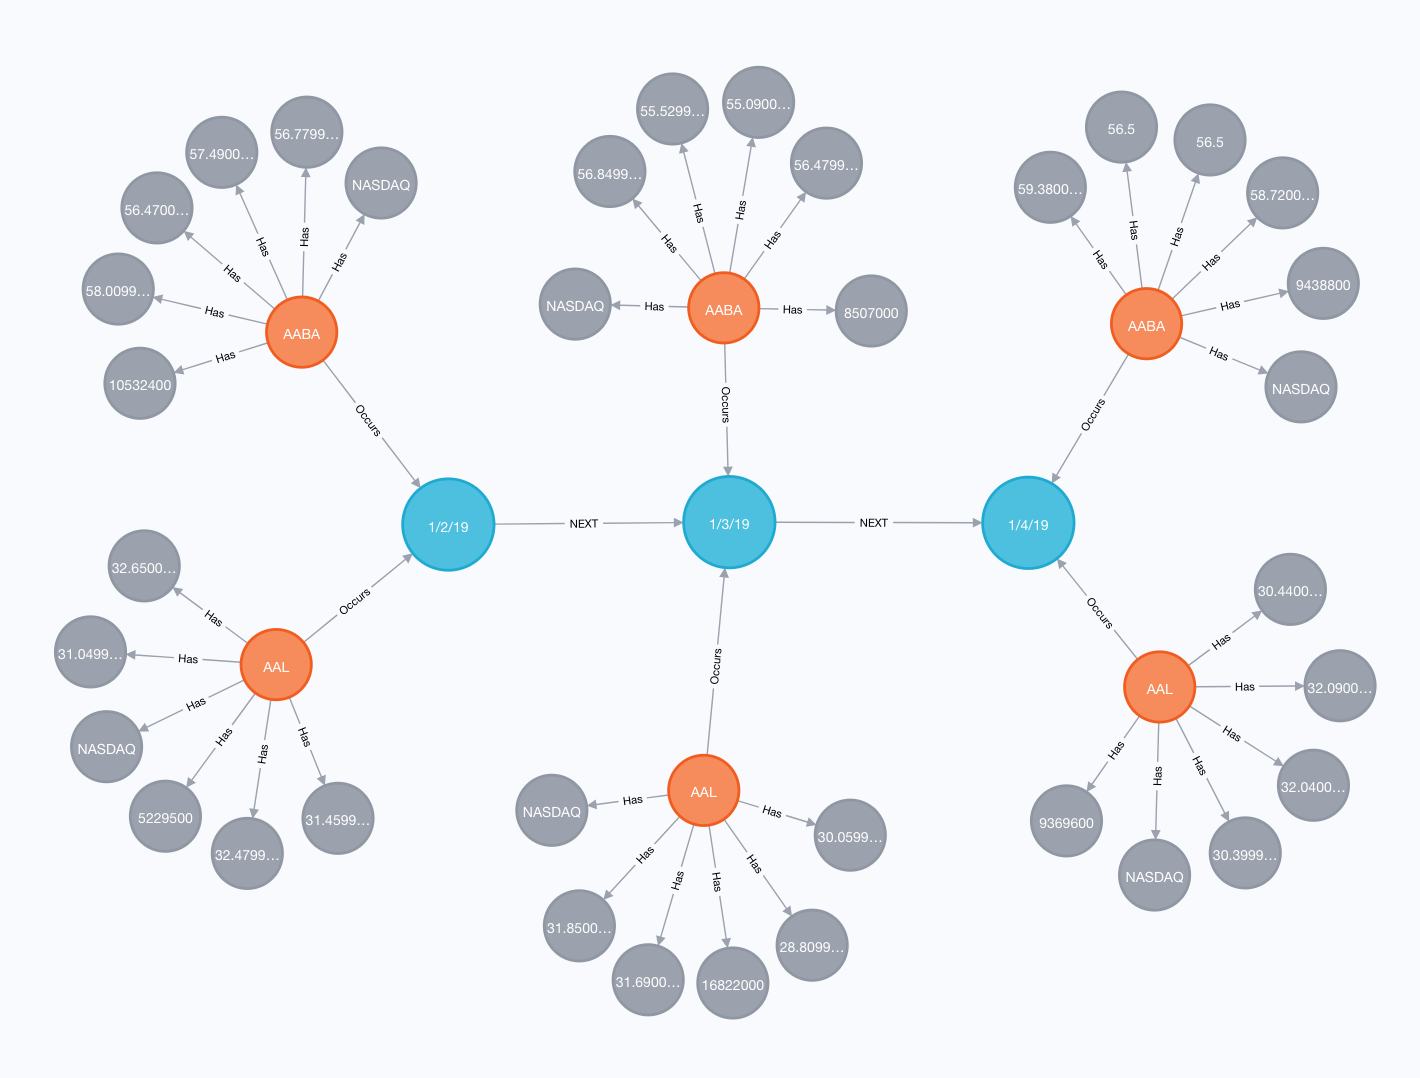
\includegraphics[width=3.5in]{Images/neo4j_data_model.png}
	\caption{Representation of sample data in Neo4j}
	\label{fig:neo4j_model}
\end{figure}

\begin{figure}
	\centering
	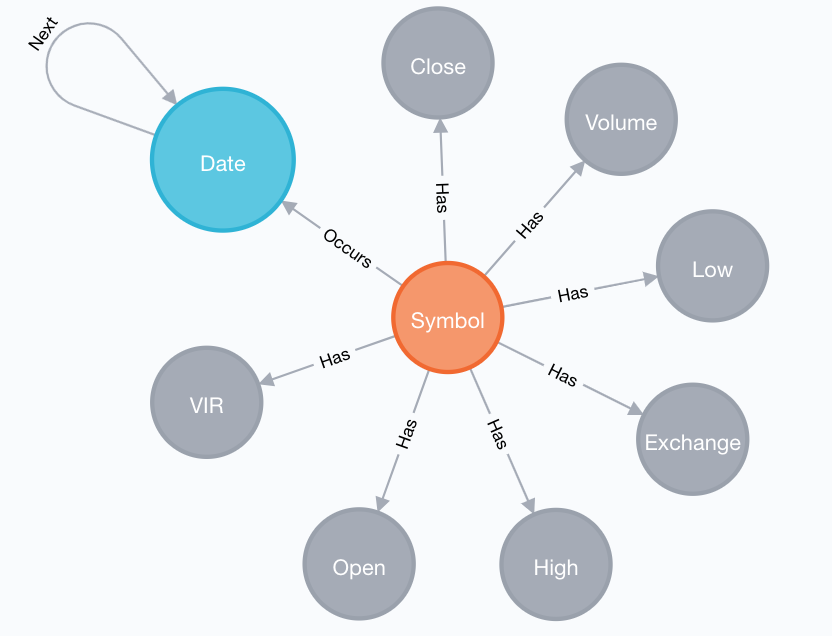
\includegraphics[width=3.5in]{Images/neo4j_general_model.png}
	\caption{Generalized data model for Neo4j}
	\label{fig:neo4j_gen_model}
\end{figure}

\subsection{VIR Calculation}

In order to make a Volatility Index calculation, we needed a minimum of twenty-two days worth of data. For this test we have collected historical daily data from September 1, 2018 through March 21, 2019. This allows us to calculate a running VIR for comparative weekly analysis of each stock from pre-2018 Q4 results until 2019 Q1 results. This provides us with a decent amount of chart data for historical comparison. 

\subsubsection{MySQL}

To complete the calculation in MySQL, the daily data stored in Amex, Nasdaq, and NYSE is queried with the start\_date field in AmxReqs, NyReqs, and NdqReqs, using a subquery of the high and close values from the corresponding table housing the exchange symbols, and based on a symbol match in the query. The start\_date field is populated based on the date\_add() function subtracting the correct amount of days.

\begin{verbatim}
-- Populate start_date field in NyReqs 
-- table to account for missing previous data 

update NyReqs set start_date = 
    date_add(date, interval -22 day);
\end{verbatim}  

The high\_high and high\_close are each calculated using a subquery of the corresponding daily table using the max() function against both high and close values.  In the example below NYSE is queried for max(high) and max(close), combined with a match on symbol in both the NYSE and the NyReqs table.  

\begin{verbatim}
-- Populate the high_high and high_close 
-- values in NyReqs from nyse table for 
-- each symbol 

update NyReqs set high_high = (select max(high) 
    from nyse as a where a.symbol=NyReqs.symbol 
    and a.date between NyReqs.date and 
    NyReqs.start_date), high_close = 
    (select max(close) from nyse as b where 
    b.symbol=NyReqs.symbol and b.date between 
    NyReqs.date and NyReqs.start_date); 
\end{verbatim}

The VIR calculation uses the calculated high\_close and high\_high values written in the previous query. The NyReqs table is updated using the set function to update the VIR field for each row based on the high\_high and high\_close assigned to the row.  

\begin{verbatim}
-- Calculate the Volatility Index Rating (VIR)  

update NyReqs set VIR = ((High_Close - close) 
    / High_High)*100; 
\end{verbatim}

\subsubsection{Neo4j}

We were able to make the VIR computation with our Neo4j database using the query language Cypher. As seen in Equation \ref{eq:vir}, the first value to be calculated is the highest close over a given 22 days. The following Cypher query obtains this value.
\begin{verbatim}
match (d:Date)-[:Occurs]-(s:Symbol)
      -[:Has]-(p:Close)  
where s.name="ACU" and d.val>="2019-01-02" 
      and d.val<="2019-01-31" 
return max(p.val) 
\end{verbatim} 

In this query, pattern-matching is performed on the nodes with Date, Symbol, and Close labels. The \texttt{where} clause filters the desired symbol and sequence of days, and the \texttt{return} statement aggregates the Close numbers and finds the maximum value. We performed similar queries to find the highest High over those days and the current Close for the final day in the sequence. Plugging these values into Equation \ref{eq:vir}, we obtained the (rounded) result $\text{VIR} = \frac{17.02 - 16.71}{17.97}\cdot 100 = 1.725\%$ for the company with the ticker symbol ACU (that is, Acme United Corporation) on January 31st, 2019.   

Our final Cypher query to obtain Volatility Index Ratings for all symbols over all valid days is quite complex, but works in a similar manner. The algorithm first pairs dates having 20 days between them. In this way, we know which days have enough preceding data to make the calculation correctly, and we know which date on which to begin the aggregation functions as well. The query then matches all the unique symbols found in the graph, so the VIR will be calculated for all companies. Next, the algorithm uses subqueries that obtain the maximum Close, current Close, and the maximum High over the paired dates for each given symbol. Finally, the VIR calculation is made from these values, and a new node is created to store the VIR value. From this intensive query, the Volatility Index computations can be made in bulk for each company and day in a given stock exchange.

\section{Performance Test Results}

Microsoft Performance Monitor was used to collect operating system (OS) statistics of overall performance for the MySQL and Neo4j queries. Metrics collected include CPU, RAM, and disk performance statistics. Additional performance metrics collected are from MySQL performance reports.  

\subsection{MySQL Results}

The system performed well when calculating the Amex high\_high and high\_close, plus the VIR calculation. CPU utilization overall averaged approximately 8\% of total CPU utilization and spiked to 80\% CPU utilization. Of that overall use approximately 14\% average CPU utilization was in the form of user time. This is good utilization of system resources since the overall interrupts and privileged times were low in comparison. Fig. \ref{fig:overall_cpu} and Fig. \ref{fig:usertime_cpu} show the overall processor utilization versus the user time utilization. They are almost directly synchronized, in contrast to privileged time which is accounting for only 2.5\% of CPU utilization, as observed from Fig. \ref{fig:privilegedtime_cpu}.  

Disk transfers and disk writes in Fig. \ref{fig:disk_transfer_write} show us the disk utilization on the system. Overall, we are using very little disk for any of the calculation. This aligns with expectations that we are mostly utilizing memory for the calculations. Memory utilization was never a factor as the system was allotted 64GB of RAM. Since the Amex dataset is so small, placing the entire contents in memory did not consume enough for the graph to show any utilization, so it is essentially a flat line. 

\begin{figure}
	\centering
	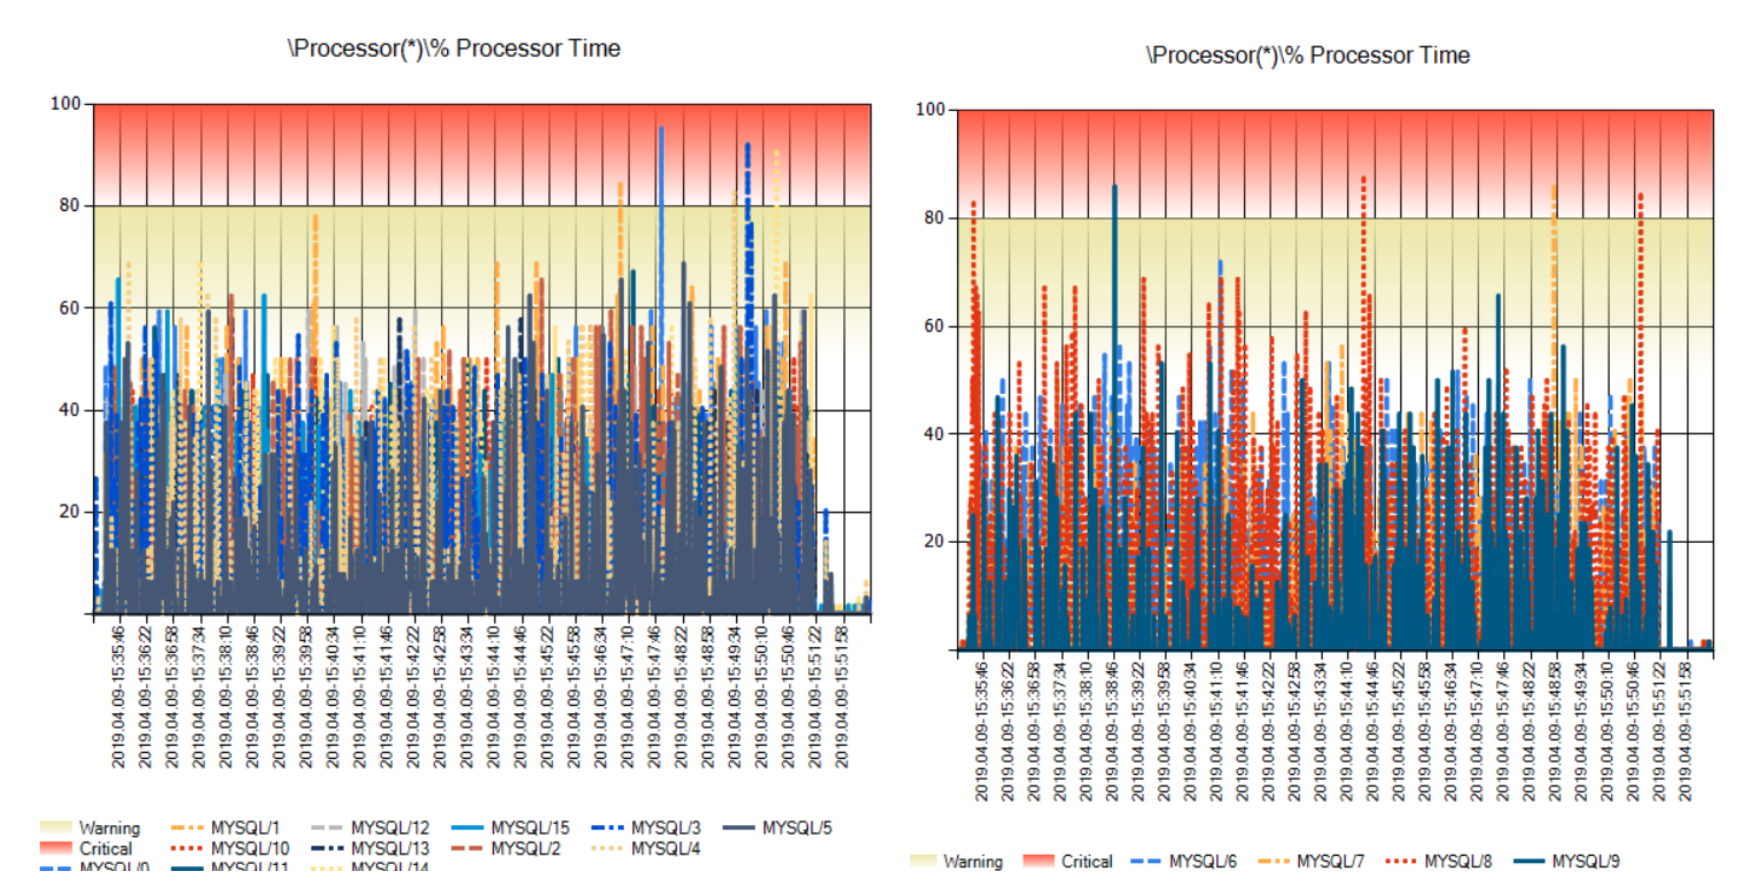
\includegraphics[width=3.5in]{Images/overall_cpu.png}
	\caption{MySQL \%Overall CPU Utilization}
	\label{fig:overall_cpu}
\end{figure}

\begin{figure}
	\centering
	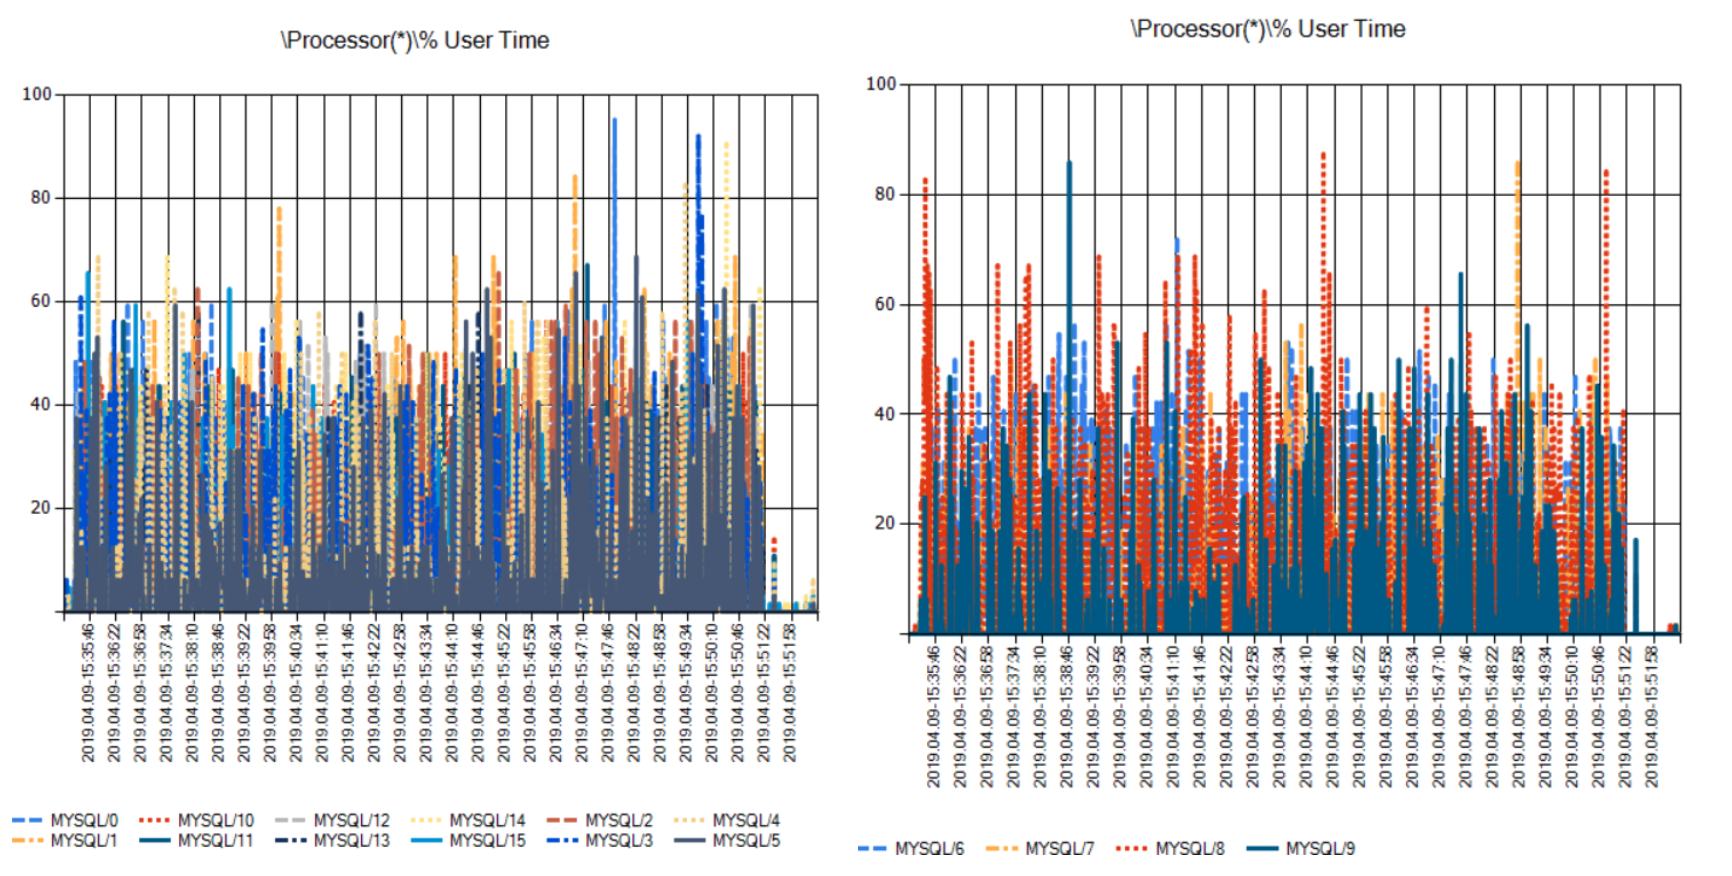
\includegraphics[width=3.5in]{Images/usertime_cpu.png}
	\caption{MySQL \%User Time CPU Utilization}
	\label{fig:usertime_cpu}
\end{figure}

\begin{figure}
	\centering
	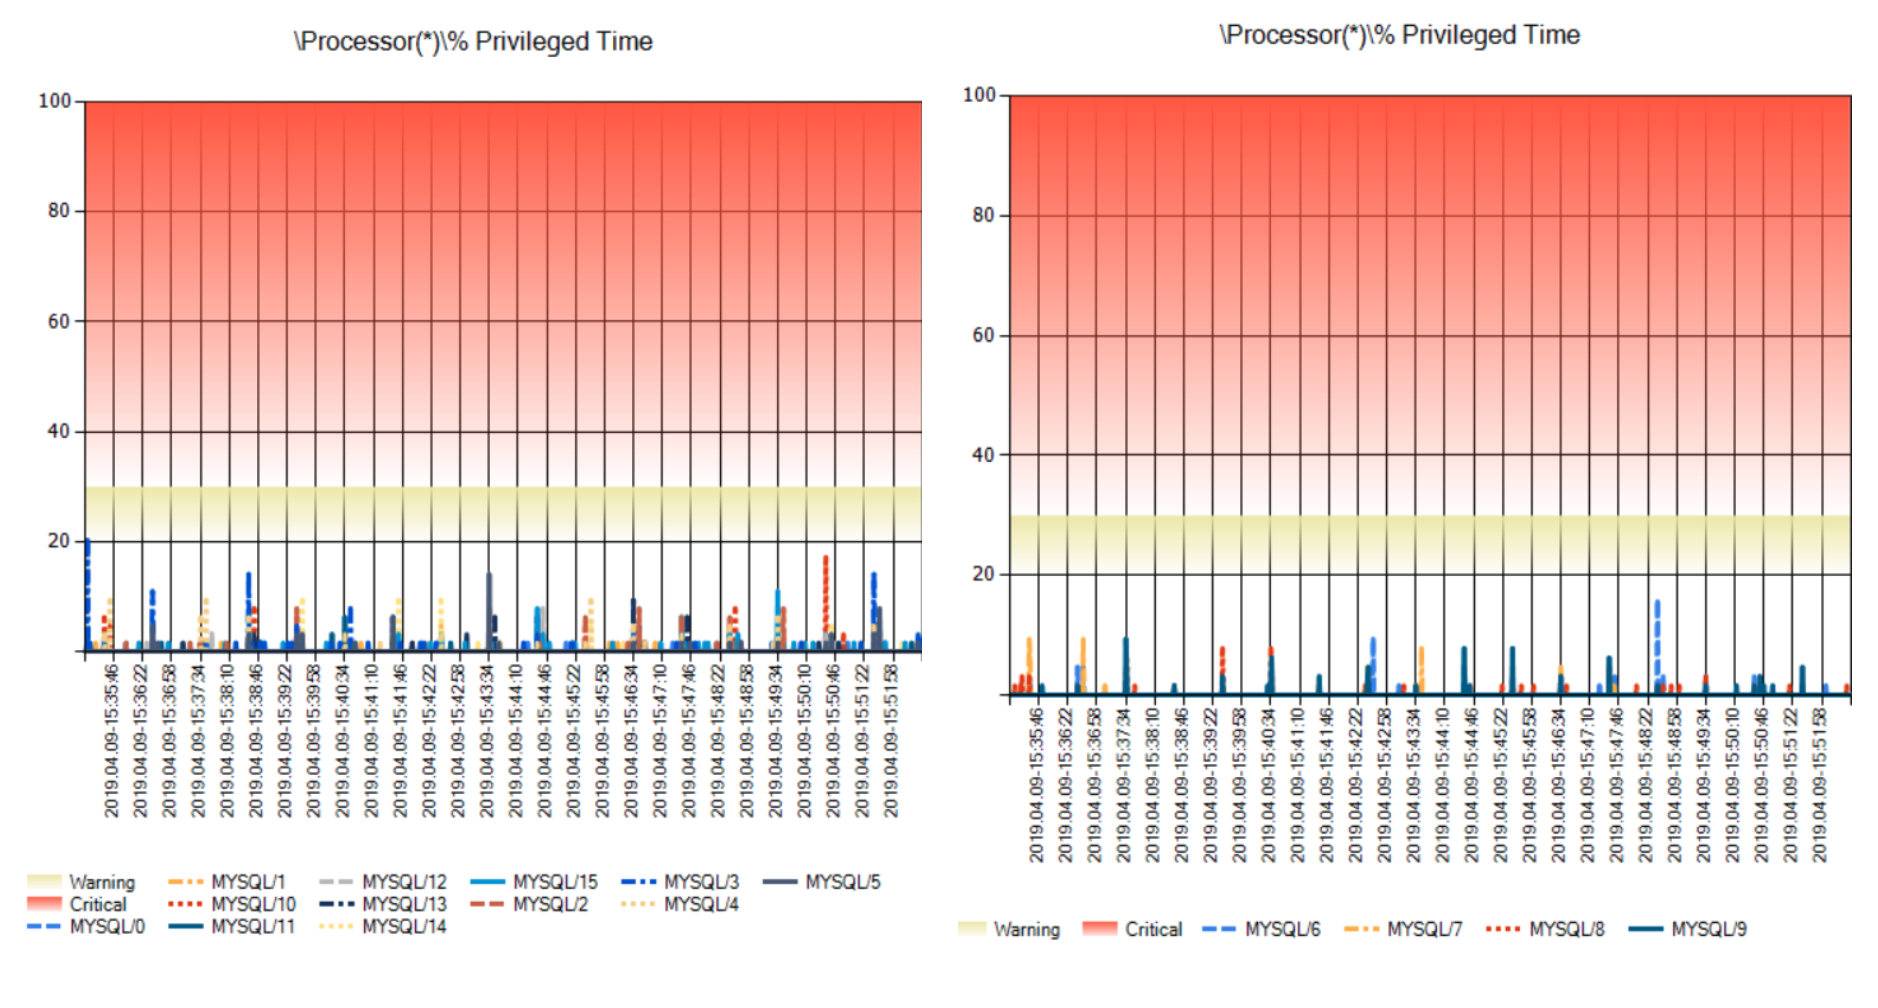
\includegraphics[width=3.5in]{Images/privilegedtime_cpu.png}
	\caption{MySQL \%Privileged Time CPU Utilization}
	\label{fig:privilegedtime_cpu}
\end{figure}

\begin{figure}
	\centering
	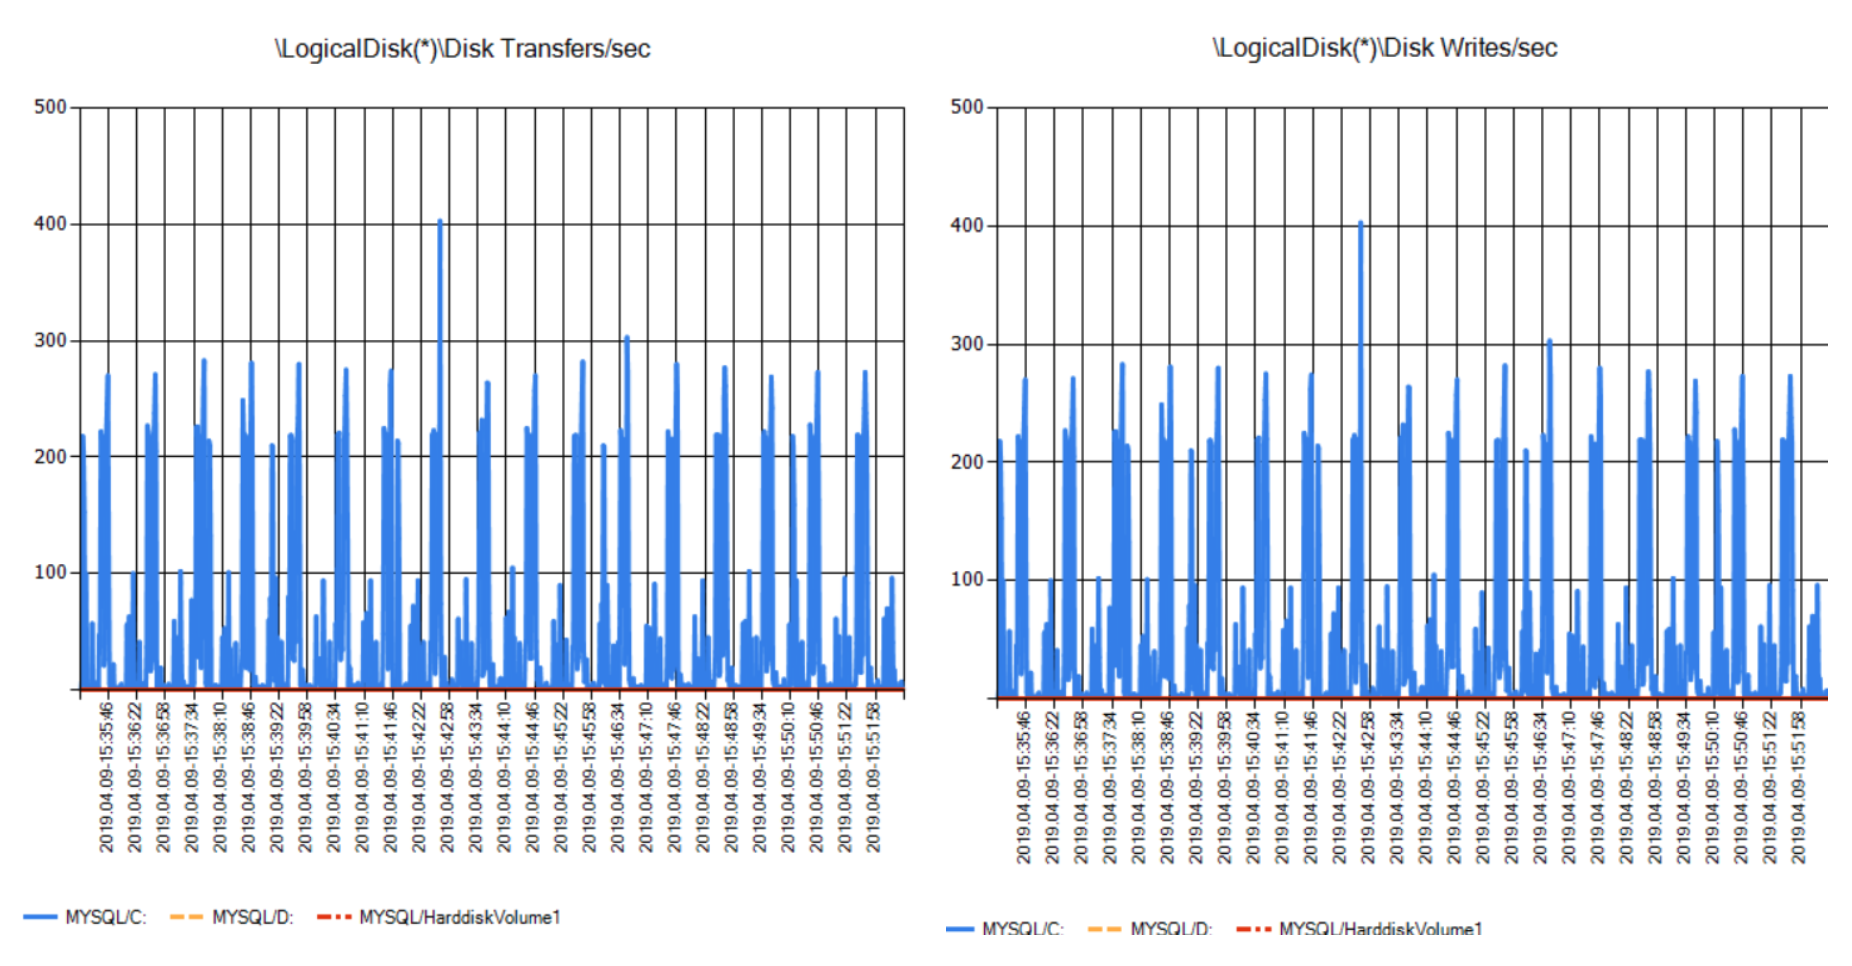
\includegraphics[width=3.5in]{Images/disk_transfer_write.png}
	\caption{MySQL Disk Transfers and Writes}
	\label{fig:disk_transfer_write}
\end{figure}

\subsubsection{MySQL Internal Statistics}

The AmxReqs start\_date query to create the start date for VIR calculations completed in 1.672 seconds, updating a total of 36,614 rows. The AmxReqs update procedure to calculate high\_high and high\_close completed in 1909.672 seconds affecting 36614 rows. The NyReqs start\_date query creating the start date for VIR calculation completed in 28.172 seconds updating 695,166 rows affected. The NyReqs update procedure to calculate high\_high and high\_close never completed. Attempts were made to set timeout values over 600k seconds, but the query failed to yield a successful result. Indexes were added to both NyReqs and NYSE. Specifically Symbol, High, and Close were indexed in NYSE and Symbol was indexed in NyReqs. No results were yielded from this change. A 600k second timeout still yielded no successful results.

\subsection{Neo4j Results}

Performing the Volatility Index calculation for only the Amex stock exchange added 31,290 labels, created 31,290 nodes, set 31,290 properties, and created 31,298 relationships in Neo4j. The query completed after 2,380,819 ms, or appropriately 40 minutes. Unfortunately, due to log file corruption, graphs of CPU and disk utilization are not available for this Neo4j query.  

When attempting to run the Cypher query on the NYSE and Nasdaq datasets, Neo4j terminated execution after around 48 hours. The server stopped due to a Java OutOfMemoryError. We found that the maximum Java heap size was set to 1GB, but increasing the heap size resulted in other errors. Time constraints did not allow for further troubleshooting of this issue.  

\section{Analysis of Results}

For the Volatility Index calculations on the Amex stock exchange, we were surprised to find that MySQL slightly outperformed Neo4j. The full computation took approximately 32 minutes in MySQL, compared to around 40 minutes in Neo4j. This is not necessarily a significant difference in times, but the results were still unexpected. We had anticipated Neo4j to greatly out-perform MySQL for this application, as related research reported that a graph database was 1,000 times faster than a relational database for their particular use case \cite{dzone}. Neo4j may have been slower due to the complexity of the query itself, or that the data was not well suited for a graph database in the first place. 

In addition, we found that the VIR calculation was too intensive of a computation for both MySQL and Neo4j when applied to a much larger dataset. Neither the NYSE or Nasdaq stock exchanges completed the calculations, even after being allowed to run for 48+ hours. MySQL timed-out after this time, and Neo4j reached its memory capacity. This could have been due to the query complexity used in both databases, as the MySQL query uses many joins and Neo4j requires an abundance of pattern matching. Nevertheless, these results lead us to believe that neither database management system or query language is appropriate for making this calculation. It is acceptable to store the stock data in either DBMS, but performing such computationally expensive queries is not fitting.  

While we initially thought that Neo4j would represent our time series data more appropriately than MySQL, through the course of our research we found that it was an awkward representation of the stock data. The data model that we created was somewhat arbitrary and subjective, because relationships between the nodes do not occur naturally. Compared to an application such as a social graph, where individuals are represented as nodes and their personal relationships between each other are conveyed, conforming the stock exchange data to a graph format felt forced. It was an interesting and valuable exercise, but overall the Neo4j representation felt unnatural for our application. Conversely, the raw stock data that we pulled in from Yahoo was already in a tabular format; from there it was natural to import it to a table in MySQL.  

\section{Future Work}

In our research, we were only able to complete VIR calculations for the Amex stock exchange, which had the smallest amount of data among the three exchanges. For both MySQL and Neo4j, the data from NYSE and Nasdaq were too large, and the VIR calculation was too computationally expensive. Both DBMSs stopped execution for these data after upwards of 48 hours; MySQL due to a time-out error and Neo4j due to a memory error. We would like to further investigate what caused the databases to fail when given such large amounts of data. We would also like to attempt query optimization to cut down on execution times for both MySQL and Neo4j.  

Regarding Neo4j in particular, we would like to investigate alternative graph databases, as research suggests it is not the most efficient graph database available \cite{graph-comp}. Previous research also indicates that Cypher can be supplemented with stored procedures to make up for some performance deficiencies \cite{graph-query}, which we could explore as another possible solution. Improvement of indexing in Neo4j could aid us as well \cite{storage-perf}. 

Additionally, since we concluded that both the relational and graph databases were inappropriate choices for making these computations, we would like to explore alternatives. In particular, we would like to explore the idea of exporting the data to Python and performing the VIR calculations there, likely using the pandas library. The Volatility calculations could then be imported back to a DBMS and be stored alongside the original data. We expect that this would be a more appropriate solution to our problem, as we would have more control of how looping and aggregation were handled in a procedural language such as Python as opposed to the declarative languages of SQL and Cypher. Either MySQL or Neo4j could still be used to store the stock data, but using them to complete the intensive computation is not optimal. 

\section{Conclusions}

The exercise of storing and manipulating the same stock exchange data in both a relational and graph database was one of value to us. We found that MySQL and Neo4j are both adequate database management systems in which to store our stock exchange data, with MySQL being a slightly more natural solution. While performing calculations on a relatively small dataset is doable for both DBMSs with comparable performance, ramping that up to much larger data is not feasible. When it comes to making intensive calculations, using a standard programming language to manipulate the data is a far better solution.  

\bibliographystyle{IEEEtran}
\bibliography{Bibliography}

\end{document}
